\documentclass{beamer}

\usepackage[utf8]{inputenc}
\usetheme{default}

\usepackage{listings}
\lstset{
basicstyle=\small\ttfamily,
columns=flexible,
breaklines=true
}

\usepackage{multicol}

 \title[66.20/86.37]{U.B.A. - Facultad de Ingeniería\\\vspace{0.25cm} 66.20/86.37 Organización de Computadoras
  \\Introducción}
  \author{Práctica jueves}
  \date{2$^{do}$ cuatrimestre 2019}


\begin{document}
\begin{frame}
\titlepage % Print the title page as the first slide
\end{frame}

\begin{frame}
 \frametitle{Docentes}
 \begin{itemize}
  \item Dr. Ing. Juan Heguiabehere\\ \href{mailto:jheguia@gmail.com}{jheguia@gmail.com}
  \item Ing. Tomás Niño Kehoe\\ \href{tomasninokehoe@gmail.com}{tomasninokehoe@gmail.com}
  \item Ing. Matias Stahl\\ \href{stahlmatias@gmail.com}{stahlmatias@gmail.com}
 \end{itemize}
\end{frame}

 \begin{frame}
 \frametitle{Temas}
 \begin{itemize}
  \item Desempeño - Ley de Amdahl
  \item ISA MIPS
  \item Jerarquía de memorias
  \item Pipeline
  \item Datapath
\end{itemize}
 \end{frame}

 \begin{frame}
 \frametitle{Evaluación}
 \begin{itemize}
\item Parcial con dos recuperatorios
\item Trabajos práctico grupal obligatorios
\item Participación en clase
\end{itemize}
 \end{frame}

\begin{frame}
 \frametitle{Herramientas}
 \begin{itemize}
  \item  Compilador: GCC
  \item Sistema de documentación: \LaTeX
  \item Emulador: QEMU
  \item Sistema de emulación gráfica MIPS: DrMIPS
  \item Sistema operativo host: Ubuntu 18.04.2 LTS 
  \item Sistema operativo guest: Debian 4.9.130-2 (2018-10-27) mips
 \end{itemize}
 \end{frame}
 
 \begin{frame}
 \frametitle{Herramientas: GCC}
 \begin{itemize} 
    \item Compilador C (entre otros)
    \item Gratuito y open source
    \item Soporta múltiples arquitecturas (inclusive MIPS)
    \item Genera código assembly
  \end{itemize}
 \end{frame}
 
\begin{frame}[fragile]
 \frametitle{Herramientas: GCC}
 Supongamos que myprog.c es el código
fuente en C a compilar:
\begin{verbatim}
$ gcc -Wall -o myexec myprog.c
\end{verbatim}

Donde:
\begin{itemize}
 \item -Wall: activa todos los mensajes de warning
\item -o: archivo de salida (en este caso, myexec)
\end{itemize}
 \end{frame}
  
 
\begin{frame}[fragile]
 \frametitle{Herramientas: GCC}
Para detener al compilador justo
después de generar el código assembly:
\begin{verbatim}
$ gcc -Wall -O0 -S  myprog.c
\end{verbatim}

Donde:
\begin{itemize}
 \item -S: detiene al compilador luego de generar el assembly
\item -O0: No aplica optimizaciones
\end{itemize}

Esto genera el archivo myprog.s con el assembly
que gcc genera para myprog.c
 \end{frame}
  

 \begin{frame}
 \frametitle{Herramientas: \LaTeX}
 \begin{itemize} 
    \item Permite concentrarse en el contenido
del documento en lugar de la forma del
mismo
    \item Formato abierto y de texto (se pueden
mantener los documentos con CVS o GIT)
    \item Resultados muy profesionales
    \item Templates tipo “paper”
  \end{itemize}

  Documentación
  \begin{itemize}
   \item “The Not So Short Introduction To LaTeX”
  \end{itemize}
  \url{http://tug.ctan.org/tex-archive/info/lshort/english/lshort.pdf}
 \end{frame}
 
  \begin{frame}
 \frametitle{Herramientas: QEMU}
Es un proyecto open source que permite emular un procesador completo incluyendo MIPS.\\~\\

\url{https://www.qemu.org/}
  \end{frame}

  
\begin{frame}[fragile]
 \frametitle{Herramientas: QEMU - Preparación del entorno}
\textit{Este entorno se prepará bajo el sistema operativo \textbf{host} Ubuntu 18.04.2 LTS}.\\~\\

 Se puede probar varias arquitecturas de MIPS utilizando una imagen de disco preconstruida con su imagen del kernel. En la máquina Host se ejecuta:
\begin{lstlisting}
$ sudo apt install qemu-system-mips
\end{lstlisting}

 \begin{lstlisting}
  wget https://people.debian.org/~jcowgill/qemu-mips/debian-stretch-mips.qcow2
  wget https://people.debian.org/~jcowgill/qemu-mips/initrd.img-4.9.0-4-5kc-malta.mips.stretch
  wget https://people.debian.org/~jcowgill/qemu-mips/vmlinux-4.9.0-4-5kc-malta.mips.stretch
 \end{lstlisting}
\end{frame}  

\begin{frame}[fragile]
 \frametitle{Herramientas: QEMU - Preparación del entorno}
Una vez finalizada la descarga de los archivos necesarios, ejecutar en el sistema Host lo siguiente:

\begin{lstlisting}
 qemu-system-mips64 \
 -M malta -cpu MIPS64R2-generic -m 2G \
 -append 'root=/dev/vda console=ttyS0 mem=2048m \
 net.ifnames=0 nokaslr' -netdev user,id=user.0 \
 -device virtio-net,netdev=user.0 \
 -net user,hostfwd=tcp::5555-:22 -net nic \
 -device usb-kbd -device usb-tablet \
 -kernel vmlinux-* -initrd initrd.img-* \
 -drive file=$(echo debian-*.qcow2),if=virtio -nographic
\end{lstlisting}

Loguearse en el sistema Guest con el usuario root (sin password).
\end{frame}  

%     \begin{frame}[fragile]
%  \frametitle{Herramientas: QEMU - Preparación del entorno} 
% \begin{figure}[h!]
%  \centering
%  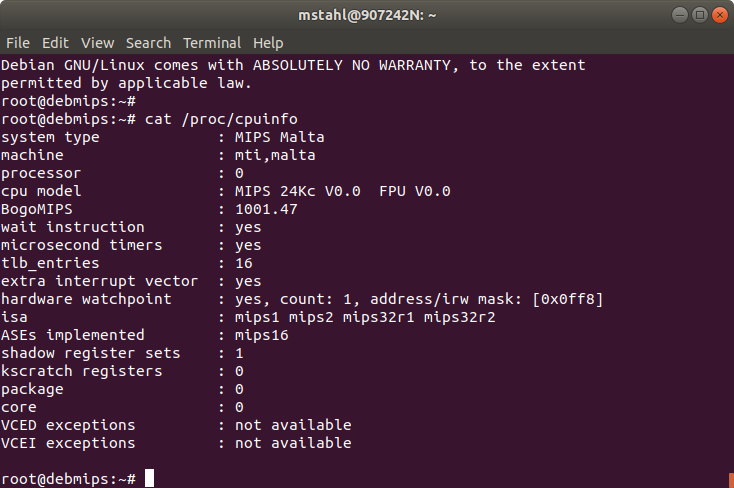
\includegraphics[scale=.4,keepaspectratio=true]{./gfx/DebianMips.png}
%  % DebianMips.png: 734x488 px, 72dpi, 25.89x17.22 cm, bb=0 0 734 488
% \end{figure} 
%   \end{frame}

\begin{frame}[fragile]
 \frametitle{Herramientas: QEMU - Instalar herramientas}
Luego de iniciar el sistema Guest, ejecutar los siguientes comandos

 \begin{lstlisting}
# dhclient
# apt-get update
# apt-get install gcc
# apt-get install gdb
# apt-get install vim
# apt-get install ssh
 \end{lstlisting}

\end{frame} 

\begin{frame}[fragile]
 \frametitle{Herramientas: QEMU - Preparación del entorno} 
 \begin{itemize}
\item Setear contraseña al usuario root
\begin{lstlisting}
# passwd root
\end{lstlisting}

\item Configurar sshd
\begin{lstlisting}
# vim /etc/ssh/sshd_config
\end{lstlisting}

Agregarle la línea \texttt{PermitRootLogin yes} y luego reiniciar el servicio de sshd

\begin{lstlisting}
# service sshd restart
\end{lstlisting}
\end{itemize}
  \end{frame}


\begin{frame}[fragile]
 \frametitle{Herramientas: QEMU - Preparación del entorno} 
 \begin{itemize}
\item Para acceder a la máquina guest desde el host
\begin{lstlisting}
$ ssh root@localhost -p 5555
\end{lstlisting}

\item Copiar archivos
\begin{lstlisting}
$ scp -P 5555 file.txt root@localhost:/tmp
\end{lstlisting}

\end{itemize}
  \end{frame}

  
  \begin{frame}[fragile]
 \frametitle{Herramientas: QEMU - Hola mundo} 
\textbf{holamundo.c}
\begin{lstlisting}
#include <unistd.h>
extern size_t mystrlen(const char *);

int main(int argc, char * const argv[]){
        char *msg = "Hola mundo.\n";
        write(1, msg, mystrlen(msg));
        return 0;
}

\end{lstlisting}
\end{frame}


  \begin{frame}[fragile]
 \frametitle{Herramientas: QEMU - Hola mundo}
 \textbf{mystrlen.S}

\begin{multicols}{2}
\begin{lstlisting}
#include <sys/regdef.h>

.text
.align 2
.globl mystrlen
.ent mystrlen

mystrlen:
.frame fp, 16, ra
.set noreorder
.cpload t9
.set reorder

subu sp, sp, 16
.cprestore 0


\end{lstlisting}

\columnbreak
\begin{lstlisting}
sw fp, 4(sp)
move fp, sp
li v0, 0

mystrlen_loop:
lb t0, 0(a0)
beqz t0, mystrlen_return
addiu a0, a0, 1
addiu v0, v0, 1
j mystrlen_loop

mystrlen_return:
lw fp, 4(sp)
addu sp, sp, 16
j ra
.end mystrlen
\end{lstlisting}
\end{multicols}
\end{frame}

  \begin{frame}[fragile]
 \frametitle{Herramientas: QEMU - Hola mundo} 
Compilar y ejecutar en el entorno guest Debian MIPS.

\begin{lstlisting}
# gcc -Wall -g -o holamundo holamundo.c mystrlen.S 
# ./holamundo 
Hola mundo.
# 
\end{lstlisting}
\end{frame}

\begin{frame}
 \frametitle{Links}
 \begin{itemize}
\item Grupo Yahoo \\ \url{https://groups.yahoo.com/neo/groups/orga6620}
\item Grupo Slack \\ \url{https://orga6620.slack.com}
 \end{itemize}
 \end{frame}

\begin{frame}
 \frametitle{Bibliografía}
 \begin{itemize}

\item David Patterson, John Hennessy, \textit{Computer Architecture a Quantitative Approach}, Elsevier, 3rd edition. ISBN: 1-55860-596-7. May 2002.  
  
\item David Patterson, John Hennessy, \textit{Computer Organization and Design, the Hardware/Software Interface},  Elsevier, 3rd edition. ISBN: 1-55860-604-1. Aug. 2004. 
    
\item B.L. Jacob and T.N. Mudge, \textit{Virtual Memory: Issues of Implementation}, Computer, Vol. 31, No. 6, June 1998, pp. 33-43.

\item B.L. Jacob and T.N. Mudge, \textit{Virtual Memory in Contemporary Microprocessors}, IEEE Micro, Aug. 1998.
\end{itemize}

\end{frame}
    
\begin{frame}
 \frametitle{Bibliografía}
 \begin{itemize}

 \item Ulrich Dreper, \textit{What every programmer should know about memory
 }
\item Jean-Loup Baer, \textit{Microprocessor Architecture. From Simple Pipelines to Chip Multiprocessors}, Cambridge University Press. ISBN-13 978-0-521-76992-1. 2010

\item Rajeev Balasubramonian and Norman P. Jouppi and Naveen Muralimanohar, \textit{Multi-Core Cache Hierarchies}, Morgan and Claypool Publishers, 2011.

\item System V Application Binary Interface, MIPS RISC Processor, 3rd Edition, The Santa Cruz Operation, February 1996 (\url{http://www.sco.com/developers/devspecs/mipsabi.pdf}).
\end{itemize}

 \end{frame}
\end{document}
